\section{Results}
\subsection{Results of the Theoretical Investigation}

\subsubsection{Sample Tables of Time vs. Lift Coefficient ($C_L$) for Bluff Body $n=2,\,6\,\text{and}\,12$}

\begin{table}[H]
	\centering
	\renewcommand{\arraystretch}{1.3}
	\begin{tabular}{|c|c|}
		\hline
		\textbf{Time (s)} & \textbf{$C_L$} \\
		\hline
		$1 \times 10^{-5}$ & $2.0946206 \times 10^{-11}$ \\
		$2 \times 10^{-5}$ & $-6.5426717 \times 10^{-12}$ \\
		$3 \times 10^{-5}$ & $-7.3241302 \times 10^{-12}$ \\
		$4 \times 10^{-5}$ & $-6.6677951 \times 10^{-12}$ \\
		$5 \times 10^{-5}$ & $-5.1304516 \times 10^{-12}$ \\
		$6 \times 10^{-5}$ & $-4.3635501 \times 10^{-12}$ \\
		$7 \times 10^{-5}$ & $-3.6837751 \times 10^{-12}$ \\
		$8 \times 10^{-5}$ & $-3.2635206 \times 10^{-12}$ \\
		$9 \times 10^{-5}$ & $-2.8660898 \times 10^{-12}$ \\
		$1.0 \times 10^{-4}$ & $-2.4321206 \times 10^{-12}$ \\
		$1.1 \times 10^{-4}$ & $-2.1246574 \times 10^{-12}$ \\
		$1.2 \times 10^{-4}$ & $-1.8807166 \times 10^{-12}$ \\
		$1.3 \times 10^{-4}$ & $-1.6461582 \times 10^{-12}$ \\
		$1.4 \times 10^{-4}$ & $-1.4100222 \times 10^{-12}$ \\
		$1.5 \times 10^{-4}$ & $-1.1994923 \times 10^{-12}$ \\
		$1.6 \times 10^{-4}$ & $-1.0306274 \times 10^{-12}$ \\
		$1.7 \times 10^{-4}$ & $-8.6746456 \times 10^{-13}$ \\
		$1.8 \times 10^{-4}$ & $-7.3730846 \times 10^{-13}$ \\
		$1.9 \times 10^{-4}$ & $-6.2413158 \times 10^{-13}$ \\
		$2.0 \times 10^{-4}$ & $-5.1195718 \times 10^{-13}$ \\
		$2.1 \times 10^{-4}$ & $-4.1747569 \times 10^{-13}$ \\
		$2.2 \times 10^{-4}$ & $-3.2864061 \times 10^{-13}$ \\
		$2.3 \times 10^{-4}$ & $-2.6866516 \times 10^{-13}$ \\
		$2.4 \times 10^{-4}$ & $-2.1575370 \times 10^{-13}$ \\
		$2.5 \times 10^{-4}$ & $-1.7389840 \times 10^{-13}$ \\
		\hline
	\end{tabular}
	\label{tab:1FaceClTable}
	\caption{Example of the first 25 values of the table produced by the simulation. Time vs. Lift Coefficient ($C_L$) for bluff body $n=2$}
\end{table}

\begin{table}[H]
	\centering
	\renewcommand{\arraystretch}{1.3}
	\begin{tabular}{|c|c|}
		\hline
		\textbf{Time (s)} & \textbf{$C_L$} \\
		\hline
		$1 \times 10^{-5}$  & $-3.3657419 \times 10^{-12}$ \\
		$2 \times 10^{-5}$  & $-1.9884762 \times 10^{-11}$ \\
		$3 \times 10^{-5}$  & $-9.3048242 \times 10^{-12}$ \\
		$4 \times 10^{-5}$  & $-4.4630770 \times 10^{-12}$ \\
		$5 \times 10^{-5}$  & $-2.0927449 \times 10^{-12}$ \\
		$6 \times 10^{-5}$  & $-7.7780466 \times 10^{-13}$ \\
		$7 \times 10^{-5}$  & $-6.0321899 \times 10^{-14}$ \\
		$8 \times 10^{-5}$  & $4.8061350 \times 10^{-13}$ \\
		$9 \times 10^{-5}$  & $7.3193765 \times 10^{-13}$ \\
		$1.0 \times 10^{-4}$ & $9.6907823 \times 10^{-13}$ \\
		$1.1 \times 10^{-4}$ & $1.1376576 \times 10^{-12}$ \\
		$1.2 \times 10^{-4}$ & $1.2174253 \times 10^{-12}$ \\
		$1.3 \times 10^{-4}$ & $1.2584116 \times 10^{-12}$ \\
		$1.4 \times 10^{-4}$ & $1.3129809 \times 10^{-12}$ \\
		$1.5 \times 10^{-4}$ & $1.3234668 \times 10^{-12}$ \\
		$1.6 \times 10^{-4}$ & $1.3258472 \times 10^{-12}$ \\
		$1.7 \times 10^{-4}$ & $1.3305942 \times 10^{-12}$ \\
		$1.8 \times 10^{-4}$ & $1.3123542 \times 10^{-12}$ \\
		$1.9 \times 10^{-4}$ & $1.2928728 \times 10^{-12}$ \\
		$2.0 \times 10^{-4}$ & $1.2666382 \times 10^{-12}$ \\
		$2.1 \times 10^{-4}$ & $1.2276206 \times 10^{-12}$ \\
		$2.2 \times 10^{-4}$ & $1.1975532 \times 10^{-12}$ \\
		$2.3 \times 10^{-4}$ & $1.1559278 \times 10^{-12}$ \\
		$2.4 \times 10^{-4}$ & $1.1103320 \times 10^{-12}$ \\
		$2.5 \times 10^{-4}$ & $1.0755046 \times 10^{-12}$ \\
		\hline
	\end{tabular}
	\label{tab:6FaceClTable}
	\caption{Example of the first 25 values of the table produced by the simulation. Time vs. Lift Coefficient ($C_L$) for bluff body $n=6$}
\end{table}

\begin{table}[H]
	\centering
	\renewcommand{\arraystretch}{1.3}
	\begin{tabular}{|c|c|}
		\hline
		\textbf{Time (s)} & \textbf{$C_L$} \\
		\hline
		$1 \times 10^{-5}$  & $-2.4598505 \times 10^{-11}$ \\
		$2 \times 10^{-5}$  & $7.6579451 \times 10^{-12}$ \\
		$3 \times 10^{-5}$  & $-2.1510813 \times 10^{-12}$ \\
		$4 \times 10^{-5}$  & $-4.4206937 \times 10^{-12}$ \\
		$5 \times 10^{-5}$  & $-2.2353308 \times 10^{-12}$ \\
		$6 \times 10^{-5}$  & $-3.6197725 \times 10^{-12}$ \\
		$7 \times 10^{-5}$  & $-2.8919916 \times 10^{-12}$ \\
		$8 \times 10^{-5}$  & $-2.1972666 \times 10^{-12}$ \\
		$9 \times 10^{-5}$  & $-1.6629472 \times 10^{-12}$ \\
		$1.0 \times 10^{-4}$ & $-1.1636706 \times 10^{-12}$ \\
		$1.1 \times 10^{-4}$ & $-7.5429574 \times 10^{-13}$ \\
		$1.2 \times 10^{-4}$ & $-4.0834742 \times 10^{-13}$ \\
		$1.3 \times 10^{-4}$ & $-1.3927346 \times 10^{-13}$ \\
		$1.4 \times 10^{-4}$ & $2.5593892 \times 10^{-13}$ \\
		$1.5 \times 10^{-4}$ & $4.2789616 \times 10^{-13}$ \\
		$1.6 \times 10^{-4}$ & $6.3422462 \times 10^{-13}$ \\
		$1.7 \times 10^{-4}$ & $5.5145736 \times 10^{-13}$ \\
		$1.8 \times 10^{-4}$ & $6.3739292 \times 10^{-13}$ \\
		$1.9 \times 10^{-4}$ & $6.7691966 \times 10^{-13}$ \\
		$2.0 \times 10^{-4}$ & $7.1047796 \times 10^{-13}$ \\
		$2.1 \times 10^{-4}$ & $7.3849782 \times 10^{-13}$ \\
		$2.2 \times 10^{-4}$ & $7.3959605 \times 10^{-13}$ \\
		$2.3 \times 10^{-4}$ & $7.3249622 \times 10^{-13}$ \\
		$2.4 \times 10^{-4}$ & $7.3044772 \times 10^{-13}$ \\
		$2.5 \times 10^{-4}$ & $7.3234202 \times 10^{-13}$ \\
		\hline
	\end{tabular}
	\label{tab:12FaceClTable}
	\caption{Example of the first 30 values of the table produced by the simulation. Time vs. Lift Coefficient ($C_L$) for bluff body $n=12$}
\end{table}

\subsubsection{Lift Coefficient ($C_L$) Over Time for each Bluff Body}

\begin{figure}[H]
	\centering
	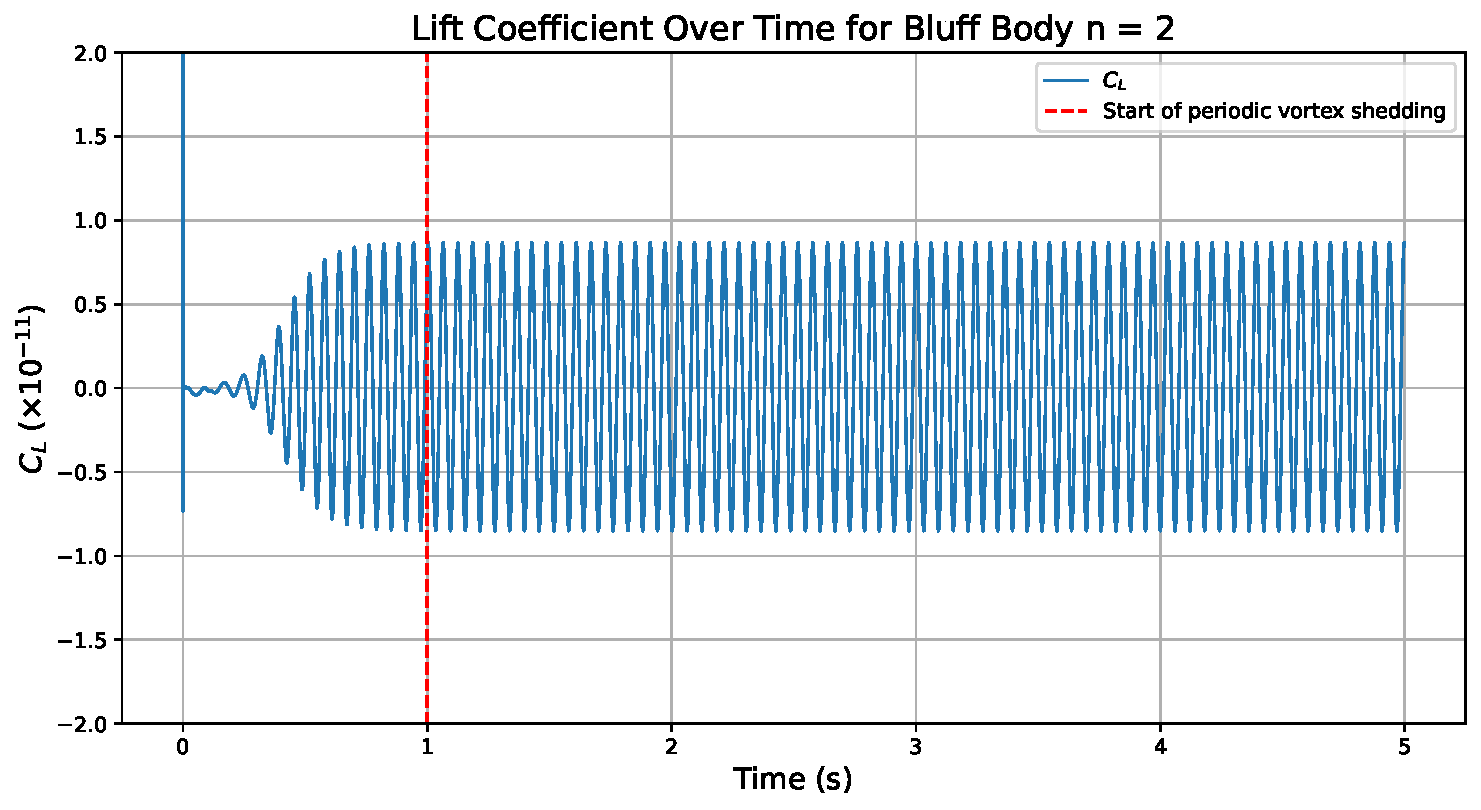
\includegraphics[width=\textwidth]{images/2face_graph}
	\caption{Lift coefficient $C_L$ over time for the bluff body $n=2$. The red dashed line indicates the start of the steady-state phase at $t = 1\,\mathrm{s}$.}
	\label{fig:2FaceGraph}
\end{figure}

\begin{figure}[H]
	\centering
	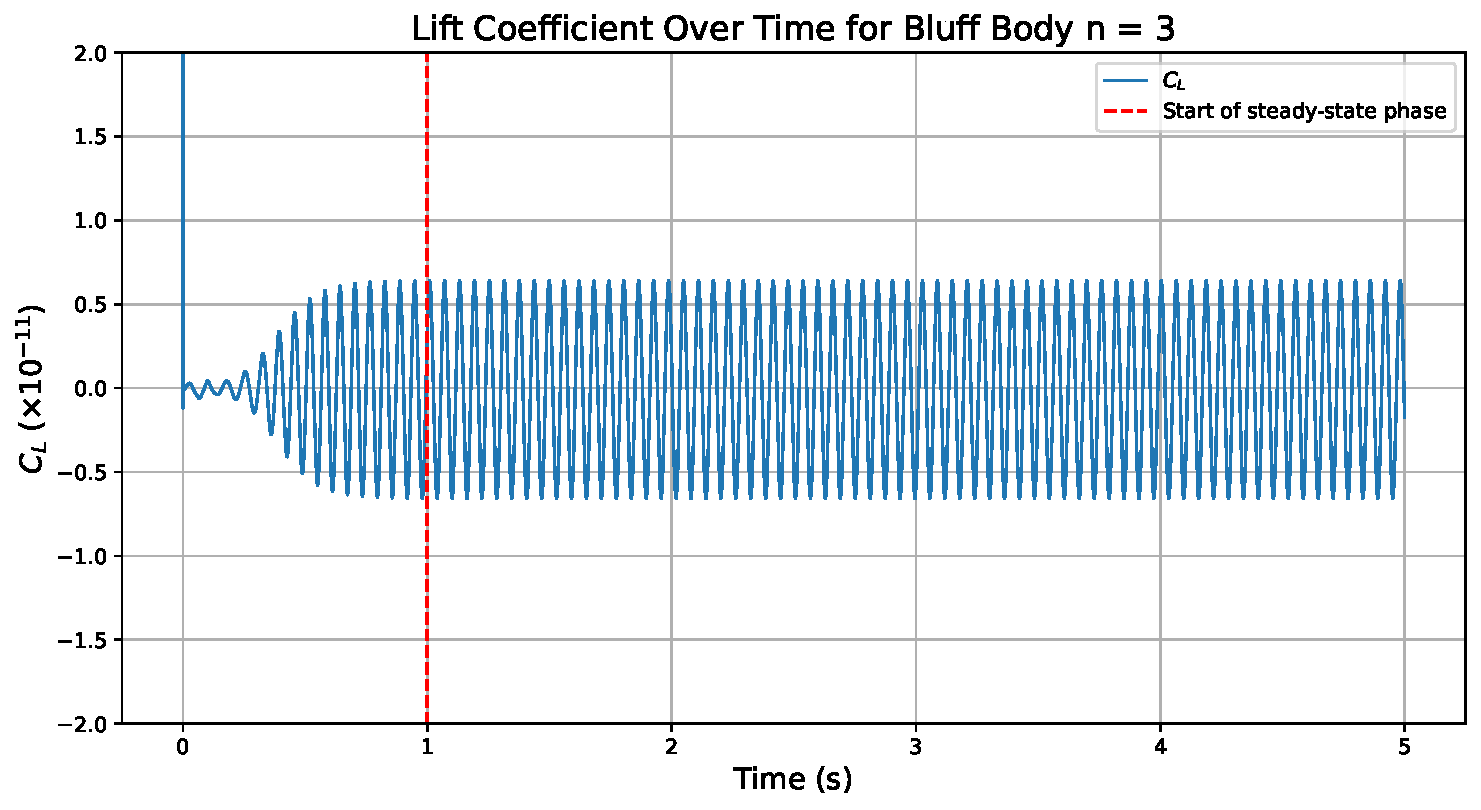
\includegraphics[width=\textwidth]{images/3face_graph}
	\caption{Lift coefficient $C_L$ over time for the bluff body $n=3$. The red dashed line indicates the start of the steady-state phase at $t = 1\,\mathrm{s}$.}
	\label{fig:3FaceGraph} 
\end{figure}

\begin{figure}[H]
	\centering
	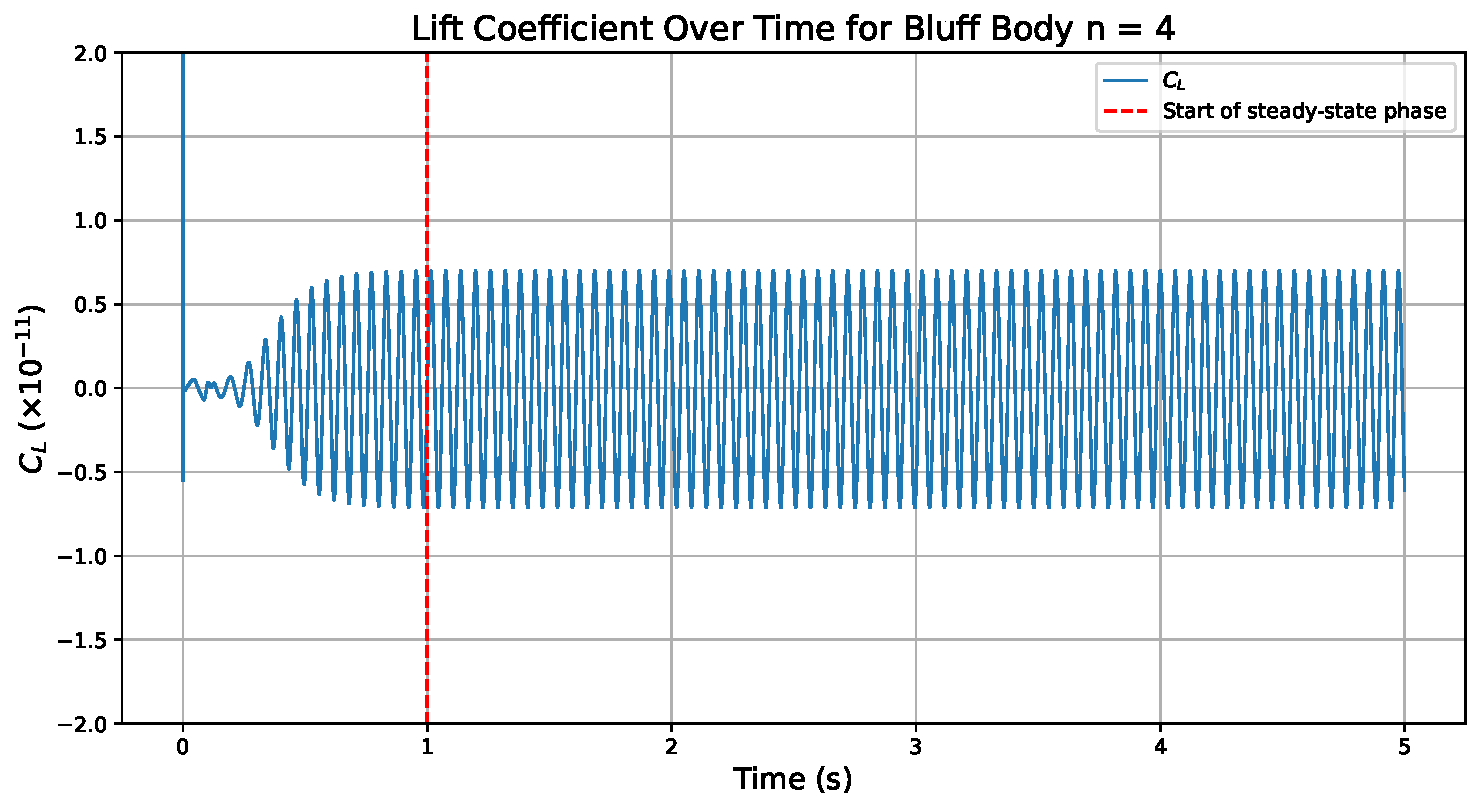
\includegraphics[width=\textwidth]{images/4face_graph}
	\caption{Lift coefficient $C_L$ over time for the bluff body $n=4$. The red dashed line indicates the start of the steady-state phase at $t = 1\,\mathrm{s}$.}
	\label{fig:4FaceGraph} 
\end{figure}

\begin{figure}[H]
	\centering
	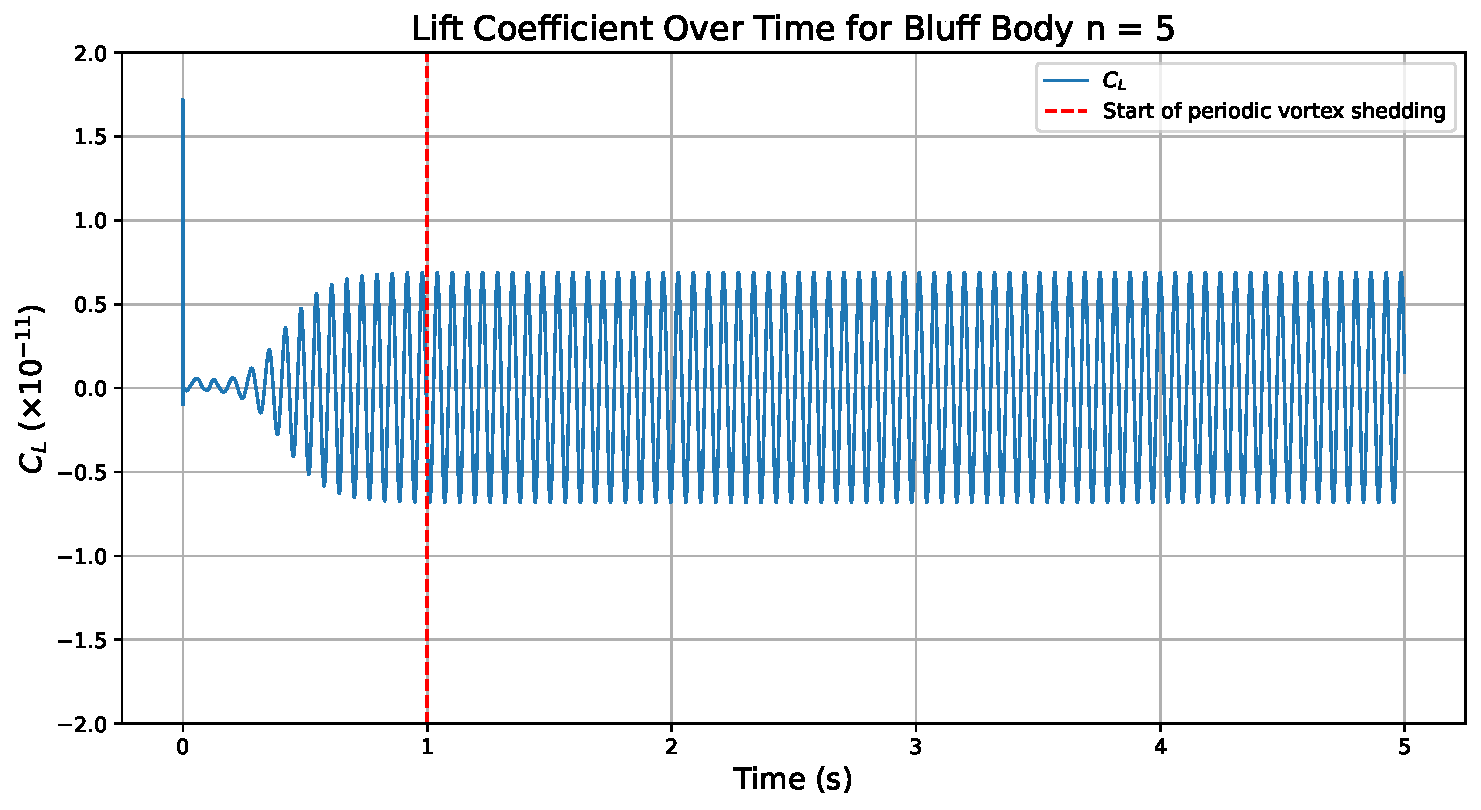
\includegraphics[width=\textwidth]{images/5face_graph}
	\caption{Lift coefficient $C_L$ over time for the bluff body $n=5$. The red dashed line indicates the start of the steady-state phase at $t = 1\,\mathrm{s}$.}
	\label{fig:5FaceGraph} 
\end{figure}

\begin{figure}[H]
	\centering
	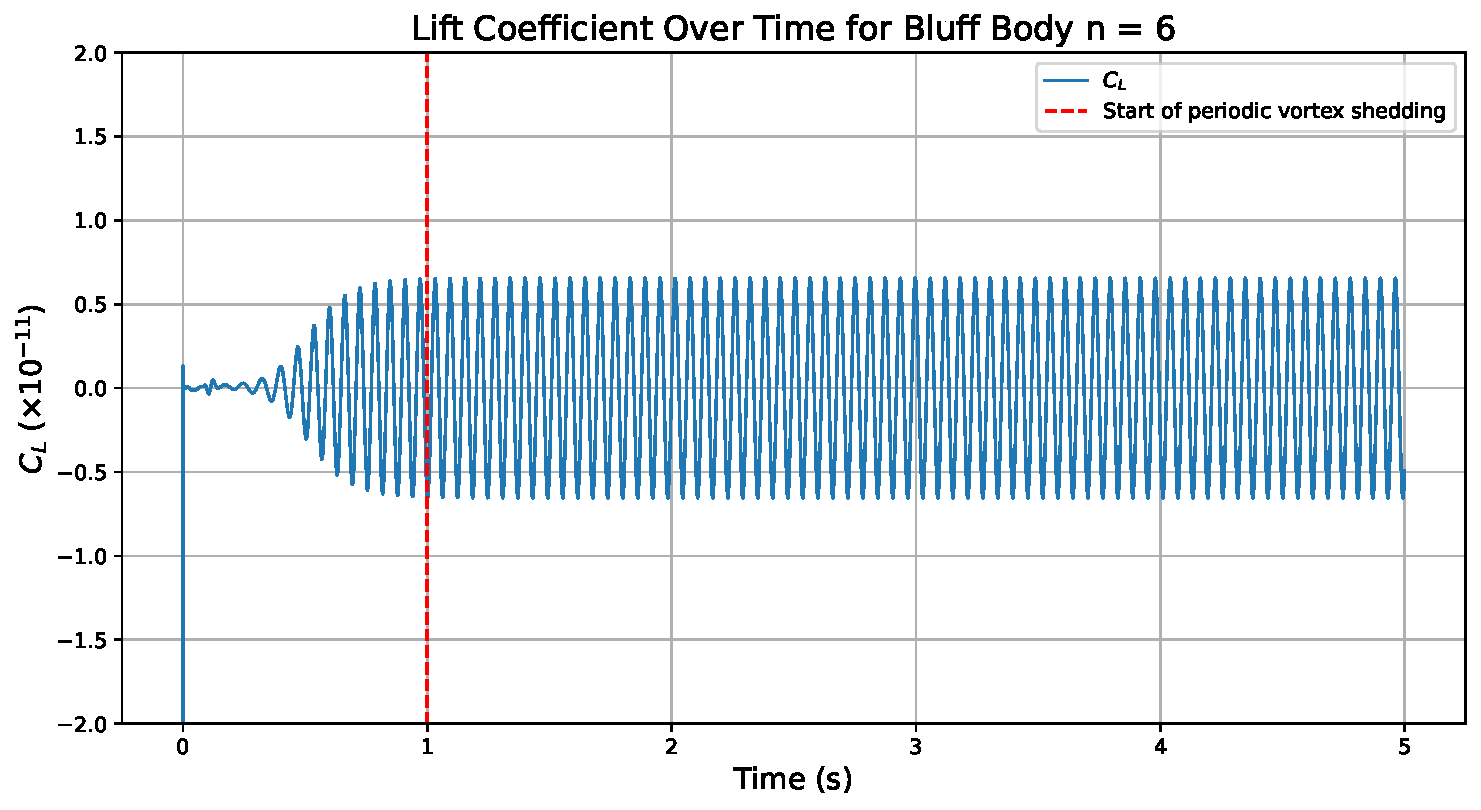
\includegraphics[width=\textwidth]{images/6face_graph}
	\caption{Lift coefficient $C_L$ over time for the bluff body $n=6$. The red dashed line indicates the start of the steady-state phase at $t = 1\,\mathrm{s}$.}
	\label{fig:6FaceGraph} 
\end{figure}

\begin{figure}[H]
	\centering
	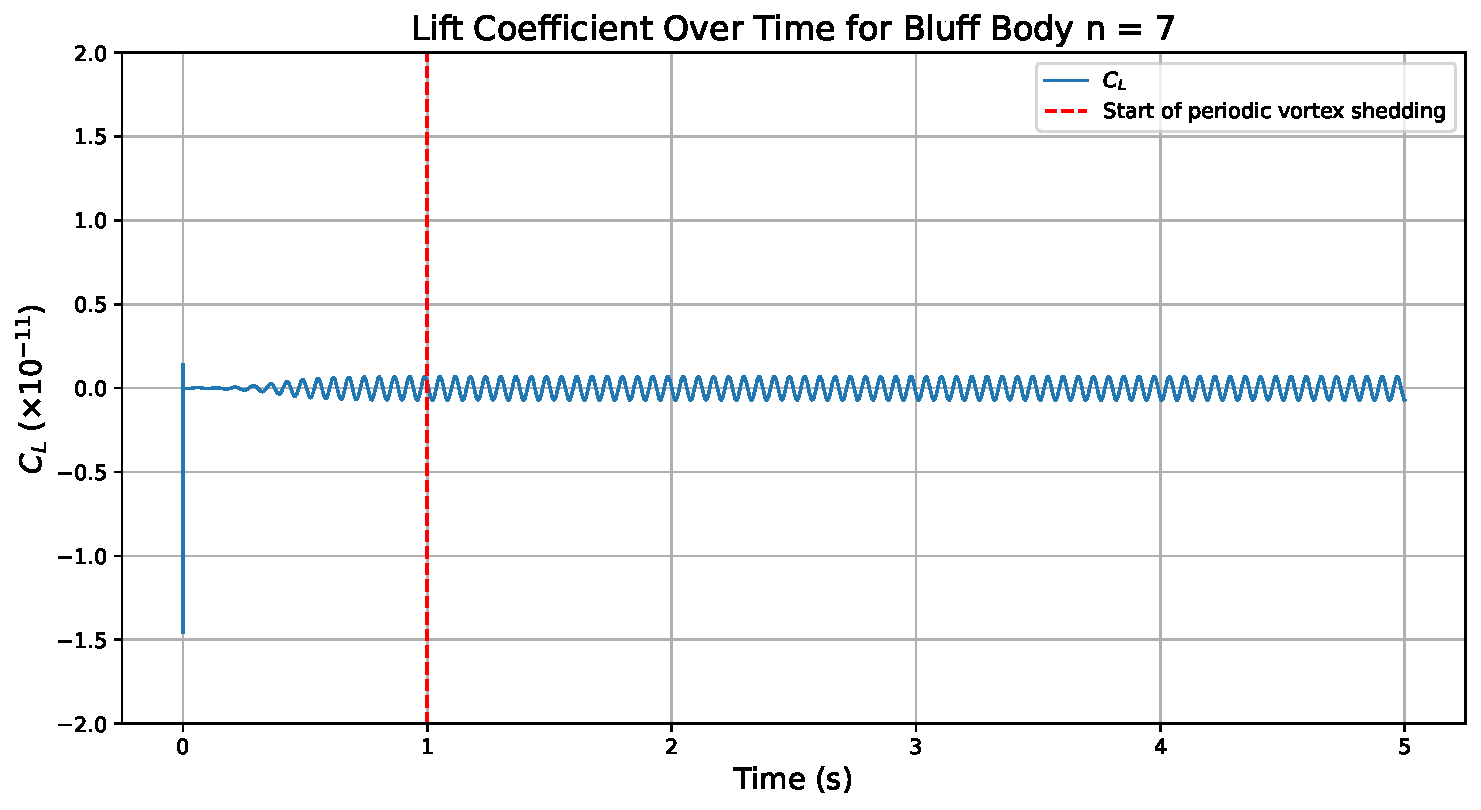
\includegraphics[width=\textwidth]{images/7face_graph}
	\caption{Lift coefficient $C_L$ over time for the bluff body $n=7$. The red dashed line indicates the start of the steady-state phase at $t = 1\,\mathrm{s}$.}
	\label{fig:7FaceGraph} 
\end{figure}

\begin{figure}[H]
	\centering
	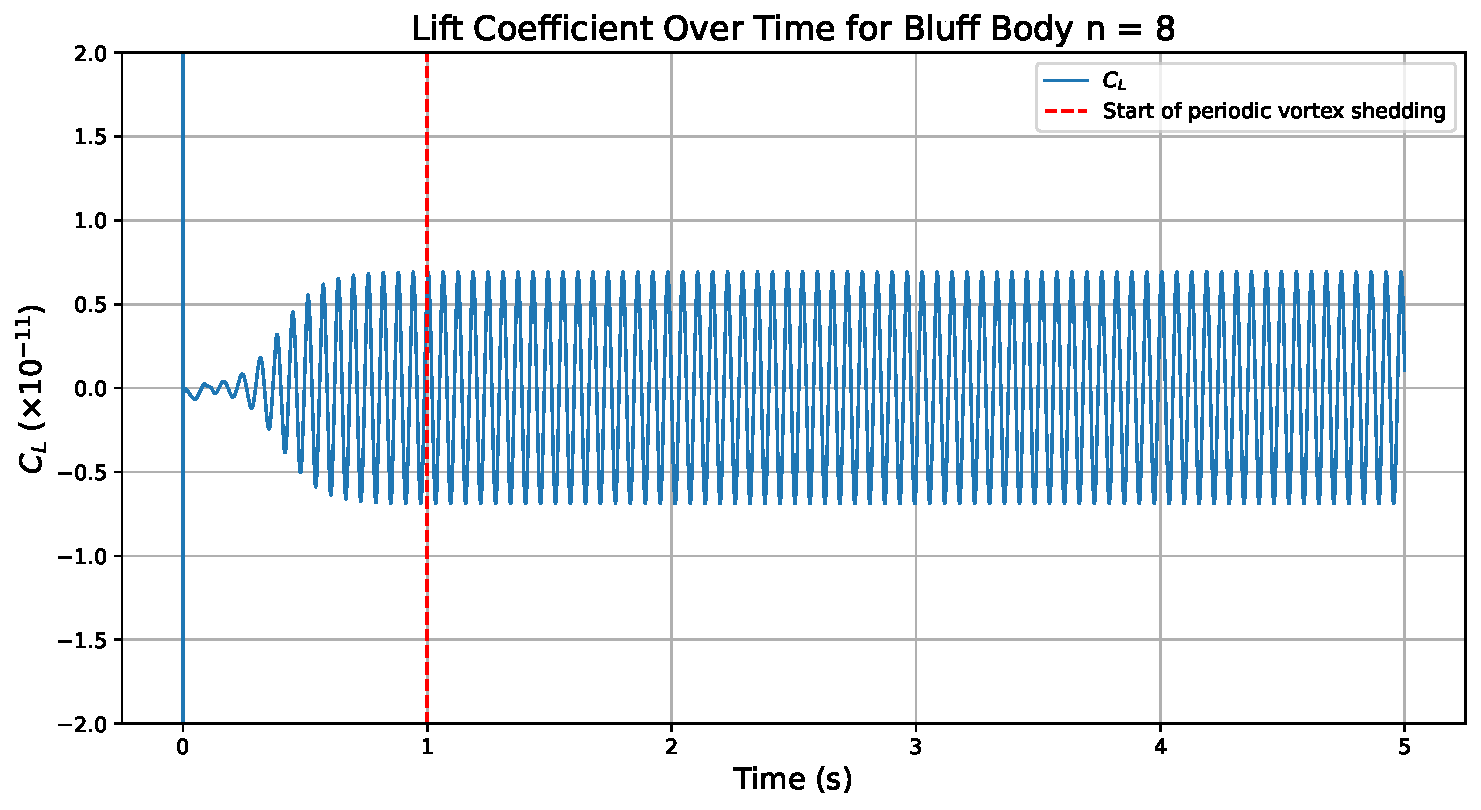
\includegraphics[width=\textwidth]{images/8face_graph}
	\caption{Lift coefficient $C_L$ over time for the bluff body $n=8$. The red dashed line indicates the start of the steady-state phase at $t = 1\,\mathrm{s}$.}
	\label{fig:8FaceGraph} 
\end{figure}

\begin{figure}[H]
	\centering
	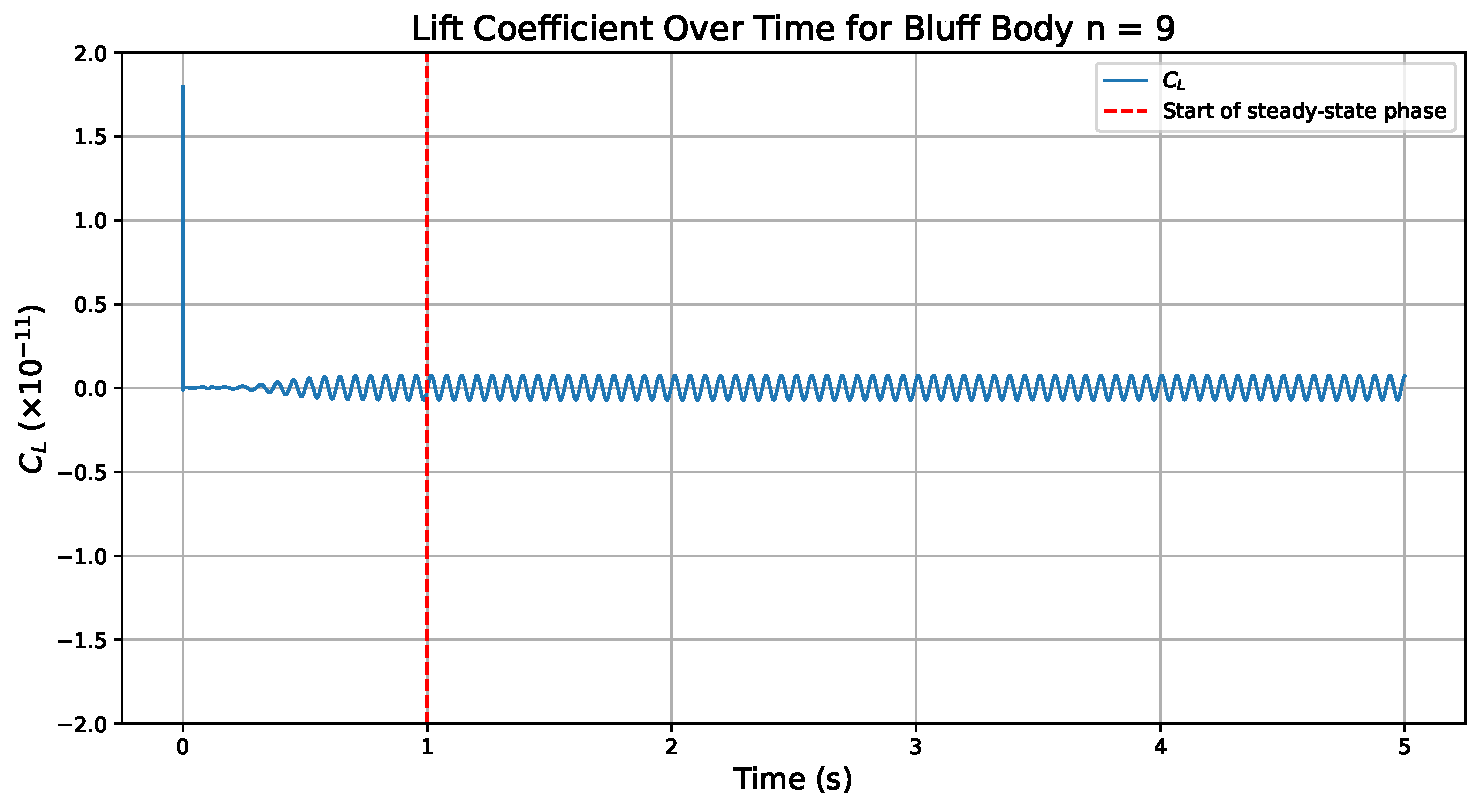
\includegraphics[width=\textwidth]{images/9face_graph}
	\caption{Lift coefficient $C_L$ over time for the bluff body $n=9$. The red dashed line indicates the start of the steady-state phase at $t = 1\,\mathrm{s}$.}
	\label{fig:9FaceGraph} 
\end{figure}

\begin{figure}[H]
	\centering
	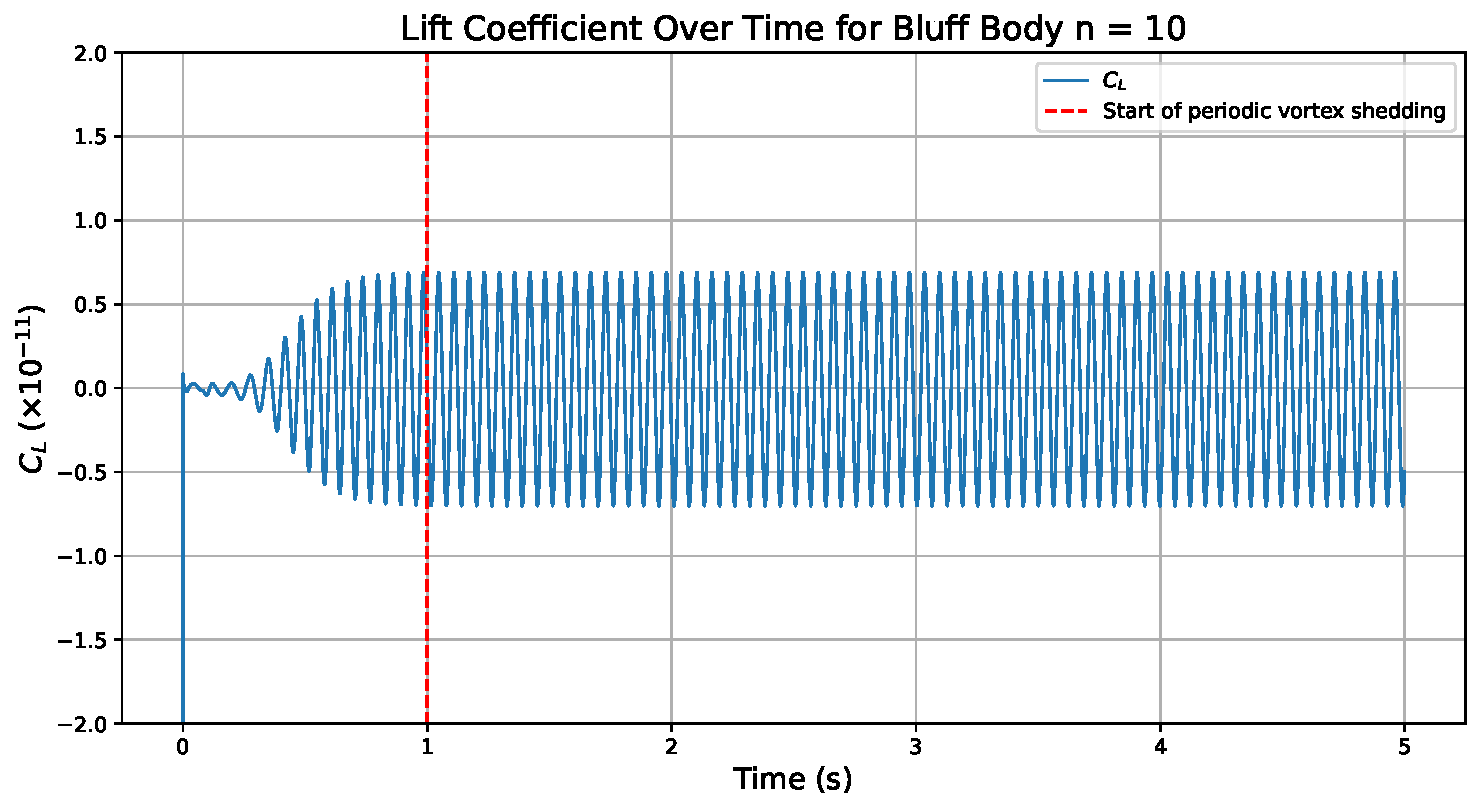
\includegraphics[width=\textwidth]{images/10face_graph}
	\caption{Lift coefficient $C_L$ over time for the bluff body $n=10$. The red dashed line indicates the start of the steady-state phase at $t = 1\,\mathrm{s}$.}
	\label{fig:10FaceGraph} 
\end{figure}

\begin{figure}[H]
	\centering
	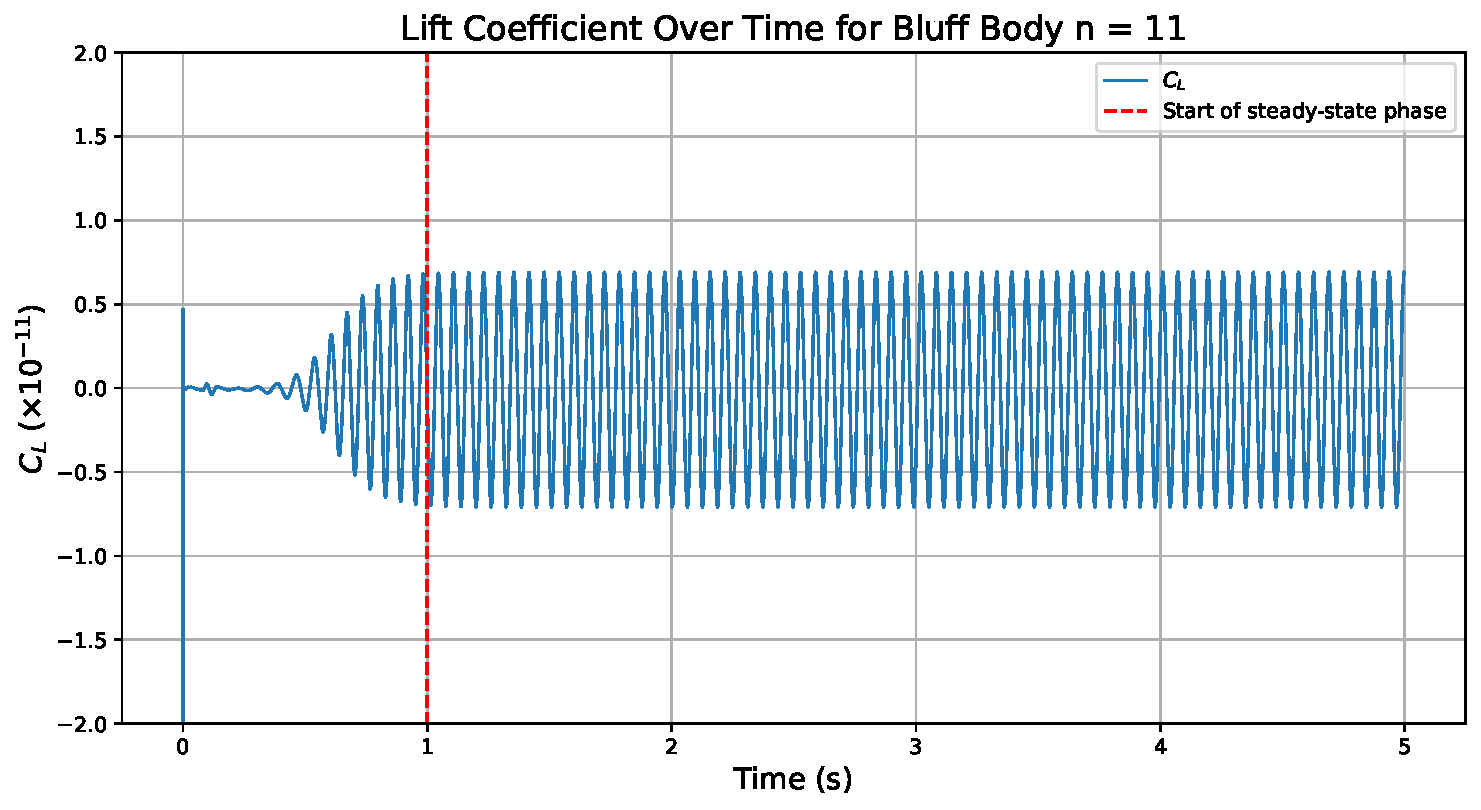
\includegraphics[width=\textwidth]{images/11face_graph}
	\caption{Lift coefficient $C_L$ over time for the bluff body $n=11$. The red dashed line indicates the start of the steady-state phase at $t = 1\,\mathrm{s}$.}
	\label{fig:11FaceGraph} 
\end{figure}

\begin{figure}[H]
	\centering
	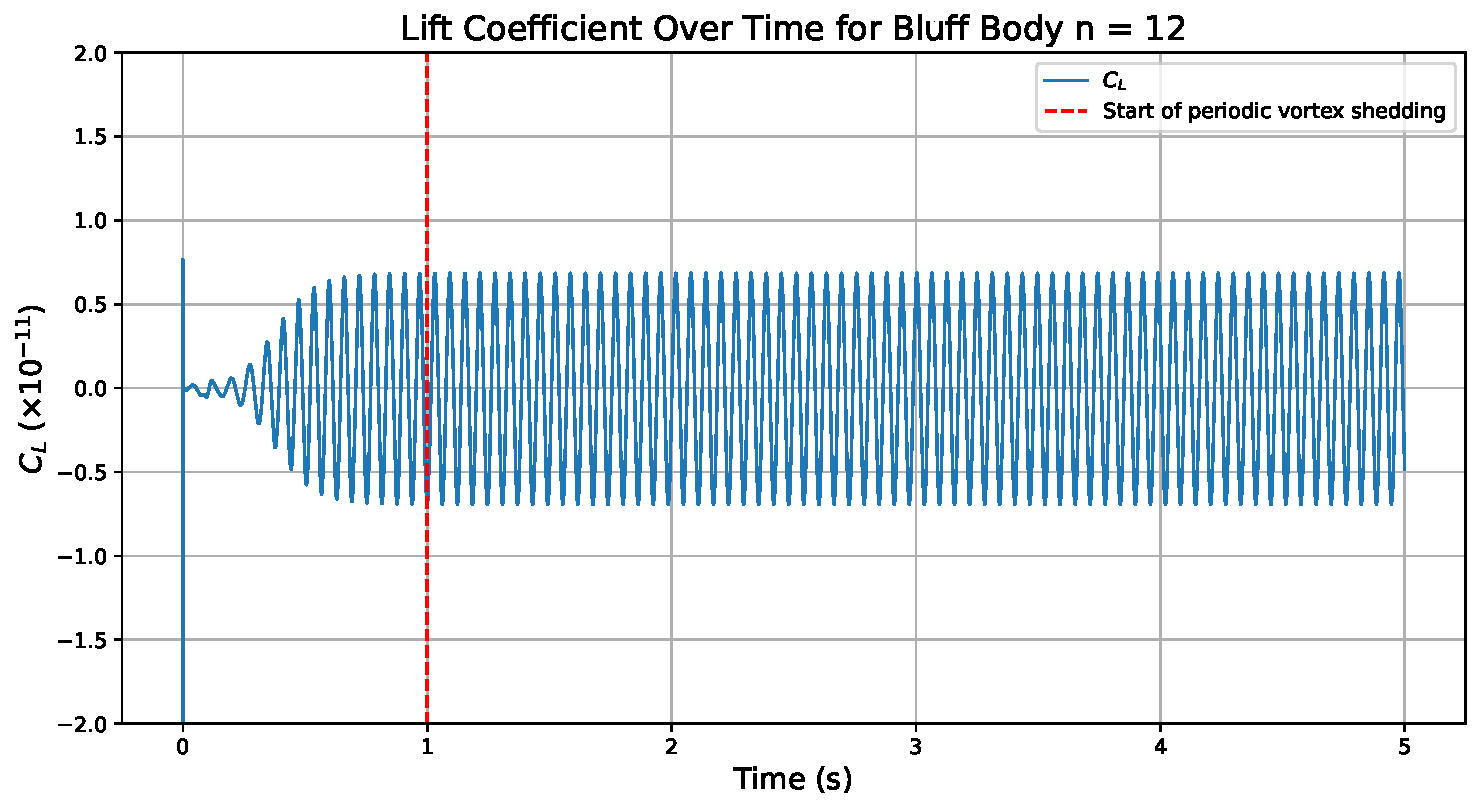
\includegraphics[width=\textwidth]{images/12face_graph}
	\caption{Lift coefficient $C_L$ over time for the bluff body $n=12$. The red dashed line indicates the start of the steady-state phase at $t = 1\,\mathrm{s}$.}
	\label{fig:12FaceGraph} 
\end{figure}

\subsubsection{Sample Calculation of Vortex Shedding Frequency for Bluff Body $n=2$ using Python}

\begin{figure}[H]
	\centering
	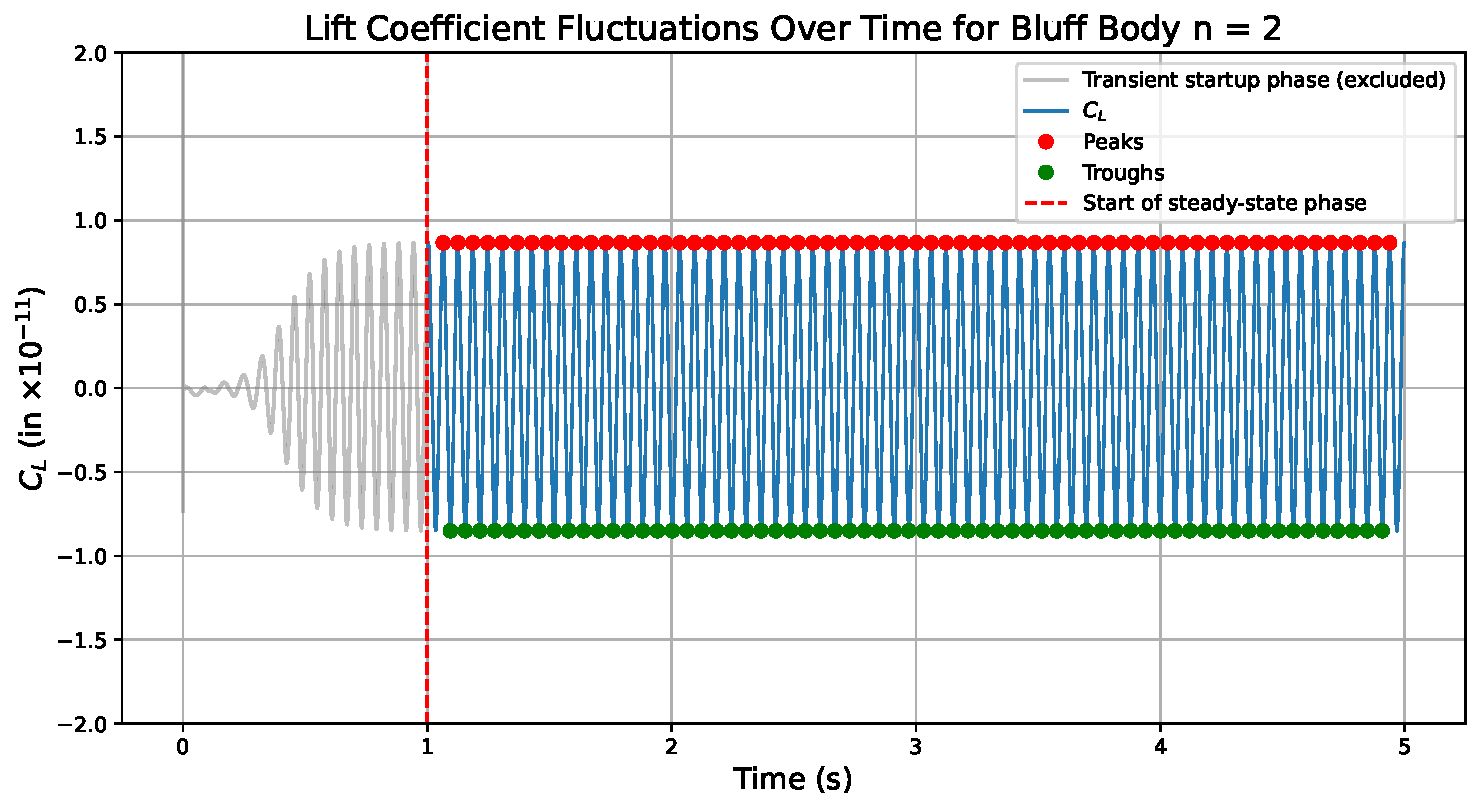
\includegraphics[width=\textwidth]{images/2face_graph_sample_Calc}
	\caption{Sample visualization of the peaks and troughs identification on the Lift Coefficient $C_L$ over time graph for bluff body $n=2$. The transient startup, colored in gray, is excluded from the detection.}
	\label{fig:2FaceGraphSampleCalc} 
\end{figure}

\begin{tcolorbox}[title=Python Output,fonttitle=\bfseries,
	colframe=black!75!white,colback=gray!10!white,boxrule=0.5pt,
	fontupper=\ttfamily]
	Number of peaks:    65 \\
	Number of troughs:  64 \\
	
	Average time period: 0.06052 s \\
\end{tcolorbox}

Using the outputted average period \( T = 0.06052 \, \text{s} \), the vortex shedding frequency was calculated with:

\[
f = \frac{1}{T} = \frac{1}{0.06052} = 16.52346 \, Hz
\]

This represents the vortex shedding frequency of the bluff body with \( n = 2 \) faces in steady-state laminar flow.

\subsubsection{A Comparison of Vortex Shedding Frequency with Increasing $n$ from 2 \textendash\ 12}

\begin{figure}[H]
	\centering
	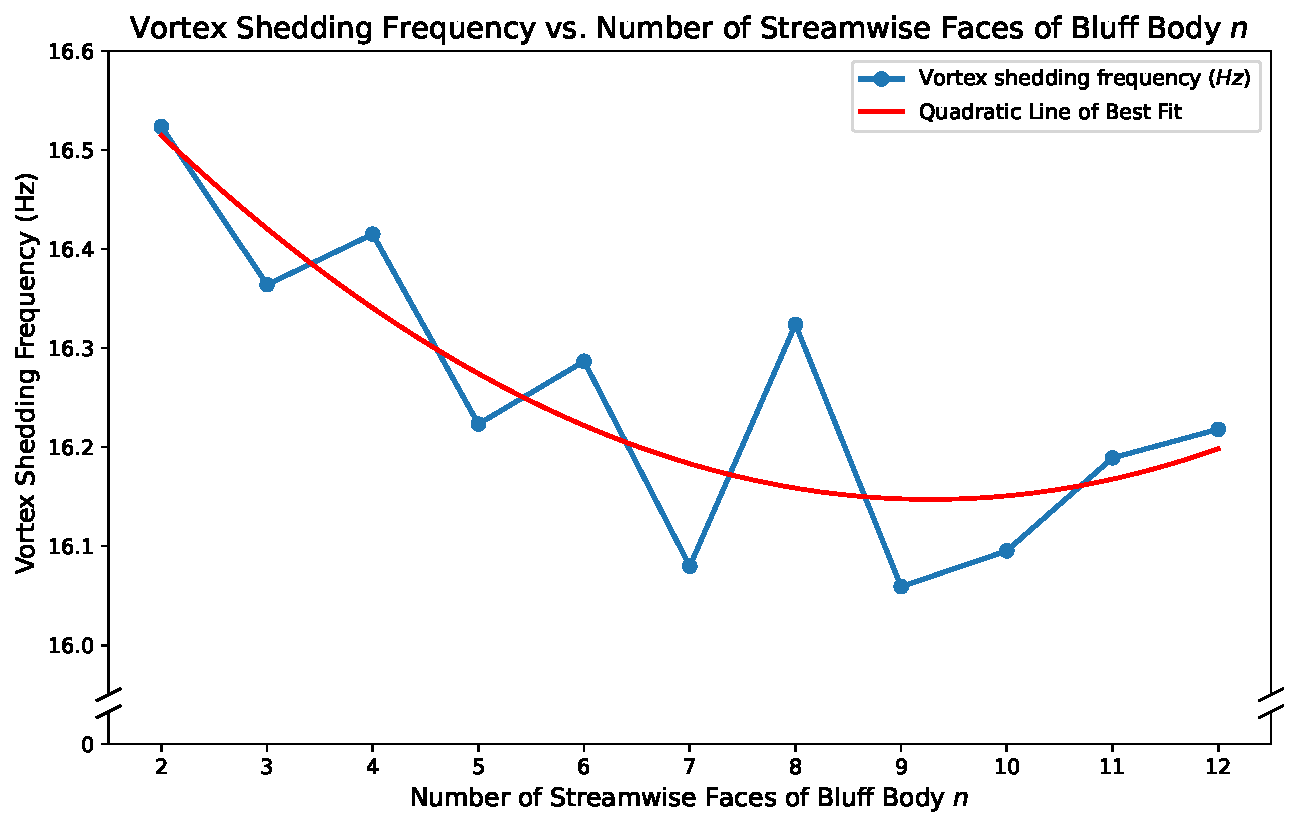
\includegraphics[width=\textwidth]{images/overall}
	\caption{A comparison of vortex shedding frequency with increasing $n$ from 2 \textendash\ 12}
	\label{fig:overall} 
\end{figure}

In order to better visualize the general non-linear trend a quadratic line of best fit was included. 


\subsection{Results of Practical Investigation}
After review of the footage it was found that the flow regime exhibited in the flow tank was not laminar. Despite many attempts to achieve laminar flow, the flow remained turbulent, as demonstrated by the irregular wake patterns. Nevertheless, the experiment yielded qualitative value. The use of potassium permanganate crystals allowed for a clear visualization of the boundary layer, flow separation and vortex shedding formation of the different bluff bodies.


	
\foreach \n in {2,...,12} {
	\subsubsection*{Snapshots of the Practical Run of Bluff Body $n = \n$}
	\begin{figure}[H]
		\centering
		
		% === Row 1 ===
		\begin{subfigure}[t]{0.48\textwidth}
			\centering
			\includegraphics[width=\linewidth]{images/\n Face/\n Face_0s.jpg}
			\caption{Snapshot of bluff body $n = \n$ at time 0 seconds}
		\end{subfigure}
		\hfill
		\begin{subfigure}[t]{0.48\textwidth}
			\centering
			\includegraphics[width=\linewidth]{images/\n Face/\n Face_1s.jpg}
			\caption{Snapshot of bluff body $n = \n$ at time 1 second}
		\end{subfigure}
		
		\vspace{1em}
		
		% === Row 2 ===
		\begin{subfigure}[t]{0.48\textwidth}
			\centering
			\includegraphics[width=\linewidth]{images/\n Face/\n Face_2s.jpg}
			\caption{Snapshot of bluff body $n = \n$ at time 2 seconds}
		\end{subfigure}
		\hfill
		\begin{subfigure}[t]{0.48\textwidth}
			\centering
			\includegraphics[width=\linewidth]{images/\n Face/\n Face_3s.jpg}
			\caption{Snapshot of bluff body $n = \n$ at time 3 seconds}
		\end{subfigure}
		
		\vspace{1em}
		
		% === Row 3 ===
		\begin{subfigure}[t]{0.48\textwidth}
			\centering
			\includegraphics[width=\linewidth]{images/\n Face/\n Face_4s.jpg}
			\caption{Snapshot of bluff body $n = \n$ at time 4 seconds}
		\end{subfigure}
		\hfill
		\begin{subfigure}[t]{0.48\textwidth}
			\centering
			\includegraphics[width=\linewidth]{images/\n Face/\n Face_5s.jpg}
			\caption{Snapshot of bluff body $n = \n$ at time 5 seconds}
		\end{subfigure}
		
	\end{figure}
}


	
	
	
	




